% !TeX root = ../main.tex
% !TeX program = xelatex
% !TeX encoding = UTF-8
\section{对照实验与机制分析}
\subsection{实测负荷的分布保真与准入}

在六栋外部计量建筑上，固定各自选取的8--10个代表日，仅比较软校正与硬能量约束下的最小Wasserstein距离权重。归一分布误差定义为一阶Wasserstein距离除以同一保留完整日序列的平均负荷。表\ref{tab:w1}列出全部六例，所示中位数仅描述这一组样本。

\begin{figure}[htbp]
\centering
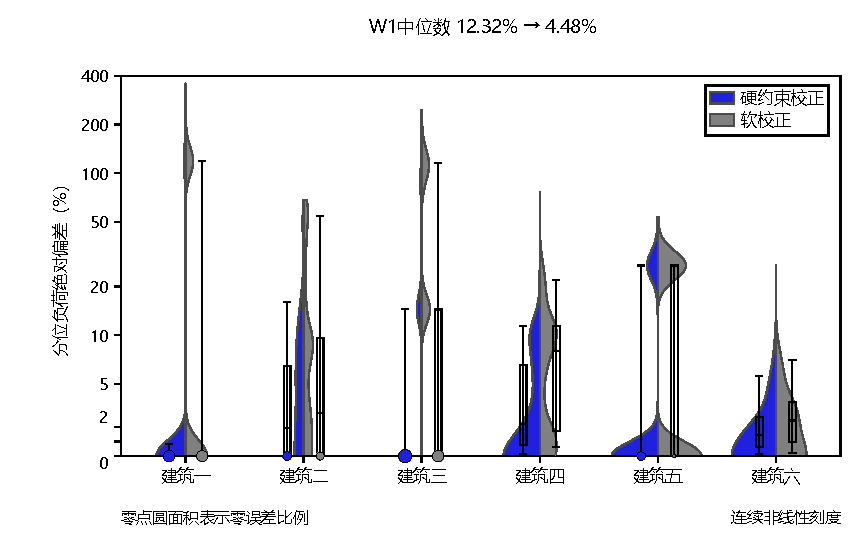
\includegraphics[width=\linewidth]{paper_r2/external_w1.pdf}
\caption{六建筑固定代表日的分布校正。蓝、灰分别表示硬约束与软校正；箱线为加权分位，零点圆面积为零偏差比例。纵轴采用连续非线性刻度，保留完整尾部。}
\label{fig:w1-distribution}
\end{figure}

图\ref{fig:w1-distribution}按相同累计概率匹配原始与代表负荷，绘制归一绝对偏差及其概率分布；箱体为25/50/75分位，须为5/95分位，均由原离散概率质量计算。加权平均偏差等于对应$W_1$，使分布形态与误差指标直接对应；小提琴轮廓仅用于密度展示。

\begin{table}[htbp]
\centering
\caption{固定代表日集合的权重校正结果}\label{tab:w1}
\begin{tabularx}{\textwidth}{@{}lrrX@{}}
\toprule
建筑 & 软校正误差/\% & 硬约束误差/\% & 硬约束候选的完整准入\\
\midrule
一 & 18.0043 & 4.8097 & 通过\\
二 & 10.0363 & 4.9463 & 原始峰值覆盖不足\\
三 & 20.9090 & 4.1453 & 新增通过\\
四 & 8.2519 & 3.8920 & 通过\\
五 & 14.5937 & 5.4303 & 原始峰值覆盖不足\\
六 & 2.7885 & 2.0065 & 通过\\
\midrule
中位数 & 12.3150 & 4.4775 & 通过数量由3/6增至4/6\\
\bottomrule
\end{tabularx}
\end{table}

六例分布误差均下降，说明相同代表日预算下的保真度得到改善。能量、峰值与爬坡门槛同时筛选规划输入，完整统计准入由3/6提高到4/6。该年度内部压缩实验表明，分布校正与极端事件检查能够互补：前者优化权重，后者保证关键负荷得到覆盖。

\subsection{厂家性能域下的固定设备调度}

对TCAV035BHE与TCAV065BHE分别登记83、82个Q/P工况点，并保留15个缺失角点。插值遵守有效单元和型号身份，对缺角、越界或跨型号查询执行拒绝。在每个城市、每个固定型号配置内，比较温控策略与条件电量费最小LP；六组对照均覆盖连续2880小时，设备台数、舒适和末状态保持相同。

\begin{table}[htbp]
\centering
\caption{同资产LP相对温控策略的条件运行收益}\label{tab:heatpump}
\begin{tabularx}{\textwidth}{@{}lXrrr@{}}
\toprule
城市 & 型号 & 降费/\% & 少付费用/元 & 增加电量/kWh\\
\midrule
乌鲁木齐 & TCAV035BHE & 1.3274 & 798.75 & 1398.80\\
乌鲁木齐 & TCAV065BHE & 1.1088 & 474.44 & 753.51\\
固原 & TCAV035BHE & 1.4526 & 908.06 & 1548.64\\
固原 & TCAV065BHE & 1.1013 & 491.80 & 874.83\\
武汉 & TCAV035BHE & 1.1268 & 173.35 & 364.93\\
武汉 & TCAV065BHE & 1.5970 & 237.79 & 728.99\\
\bottomrule
\end{tabularx}
\end{table}

表\ref{tab:heatpump}为固定资产LP数值最优解，求解界按登记编码模型核验。六例通过移时降费1.1013\%--1.5970\%，同时增加电量及固定平均因子碳排，揭示价格激励与能效目标的差异。Q/P有效域保留工况对能力的影响，理想小时占空比刻画可调度空间。

\subsection{热容与区域配电约束的交互}

为独立识别建筑热容效应，保留两个建筑的温度状态。建筑A固定$H=0.1043$~kW/K、$C=0.535576$~kWh/K；建筑B固定$H=0.15645$~kW/K，仅将$C$从0.535576改为2.142304~kWh/K。另一实验轴为是否施加6.4796375~kW的共同用电上限。四案均使用同一武汉气象、2880小时、既有理想设备和20--27~$^\circ$C服务边界。

\begin{table}[htbp]
\centering
\caption{热容倍率与公用电上限的二维对照}\label{tab:factorial}
\begin{tabularx}{\textwidth}{@{}Xrrrr@{}}
\toprule
研究设置 & 电量费/元 & 用电/kWh & 峰值/kW & 绑定小时\\
\midrule
原热容，无公用上限 & 5918.14 & 8155.11 & 14.1064 & ---\\
四倍热容，无公用上限 & 5490.94 & 8725.44 & 25.3335 & ---\\
原热容，有公用上限 & 5937.64 & 8050.61 & 6.4796 & 125\\
四倍热容，有公用上限 & 5660.96 & 8386.07 & 6.4796 & 530\\
\bottomrule
\end{tabularx}
\end{table}

四案均得到求解器容差内最优解，保存的MIP gap为0。共同上限下，增大热容使电量费下降276.68元，即4.6597\%；无共同上限时下降427.20元，即7.2185\%。两者之差150.52元量化了配电约束对热容经济价值的影响。共同上限下，区域用电增加335.46~kWh；独立积分账本将其分解为建筑A热损减少53.94~kWh与建筑B热损增加389.40~kWh，解释预热移时的能量代价。

\begin{figure}[htbp]
\centering
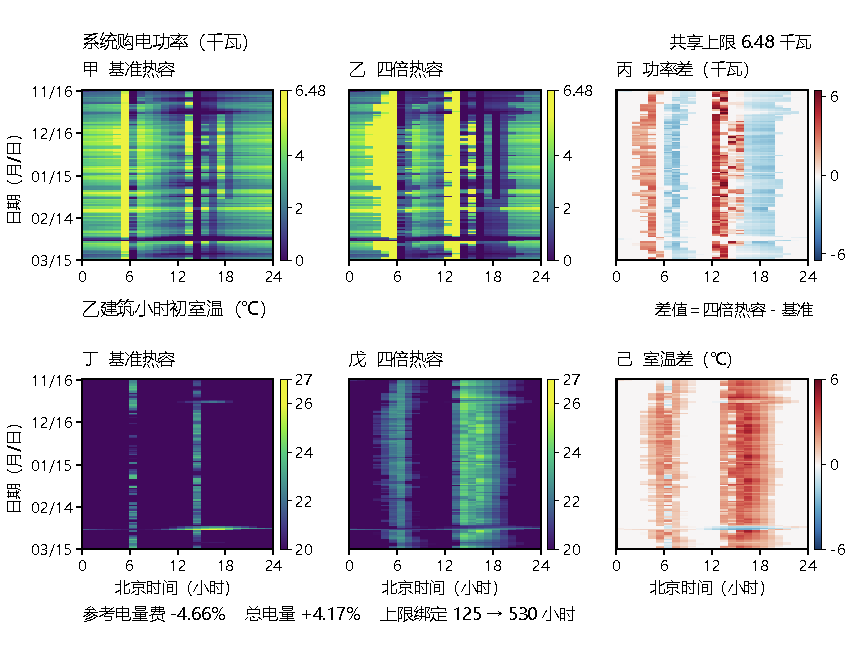
\includegraphics[width=\linewidth]{paper_r2/mechanism_paper/thermal_coupling.pdf}
\caption{共享配电边界下的热惯性调度。上排为系统购电功率，下排为乙建筑小时初室温；第三列为四倍热容减基准。图示完整120日逐时状态，显示预热时移及其容量占用。}
\label{fig:thermal-coupling}
\end{figure}

图\ref{fig:thermal-coupling}将预热与购电时移对应起来：用户热状态通过区域电力上限影响系统费用，热容价值取决于共享约束。该对照识别区域—建筑层的交互，城市级容量选择由规划接口承载。

\subsection{管网校核反馈与可行性成本}

在72小时参考系统上，对优化输出逐支路检查压降梯度、远端供水温度及热量账本。发现不满足阈值的模式后，排除该模式并重新优化。三轮对同一交付热量191.5475~kWh的结果见表\ref{tab:network}。

\begin{table}[htbp]
\centering
\caption{有限网络模式反馈的三轮结果}\label{tab:network}
\begin{tabularx}{\textwidth}{@{}Xrrr@{}}
\toprule
指标 & 第一轮 & 第二轮 & 第三轮\\
\midrule
最大压降梯度/(Pa/m) & 1081.42 & 504.33 & 237.96\\
最低远端供水温度/$^\circ$C & 61.52 & 59.85 & 57.45\\
管路热损/kWh & 35.70 & 56.94 & 94.44\\
泵耗/kWh & 0.7101 & 0.3570 & 0.1901\\
参考费用/元 & 178.64 & 195.01 & 224.26\\
校核结论 & 压降超限 & 压降超限 & 通过\\
\bottomrule
\end{tabularx}
\end{table}

第三轮满足压降梯度不大于300~Pa/m、远端供水不低于55~$^\circ$C的阈值，得到参考运行费用224.26元的可行方案。模式调整降低泵耗与压降，同时增加热损和源需求，对应费用增加25.54\%。失败模式排除与重求解自动完成这一修正，使温压可行性与其费用代价共同进入方案选择。

\subsection{三城费用—碳排取舍}

三城固定理想资产小原型以同一温控反馈策略为基准，求电量费端点、碳端点及中点碳帽。资产与厂家热泵实验不同，表\ref{tab:tradeoff}比较各自基准下的增排与降费取舍。

\begin{table}[htbp]
\centering
\caption{三城中点碳帽方案的决策取舍}\label{tab:tradeoff}
\begin{tabular*}{\textwidth}{@{\extracolsep{\fill}}lrrrr@{}}
\toprule
城市 & 费用端降费/\% & 中点降费/\% & 中点增排/\% & 降费保留/\%\\
\midrule
乌鲁木齐 & 1.7012 & 1.3916 & 1.7716 & 81.80\\
固原 & 1.7168 & 1.3892 & 1.7469 & 80.92\\
武汉 & 1.7518 & 1.5668 & 2.2003 & 89.44\\
\bottomrule
\end{tabular*}
\end{table}

\begin{figure}[htbp]
\centering
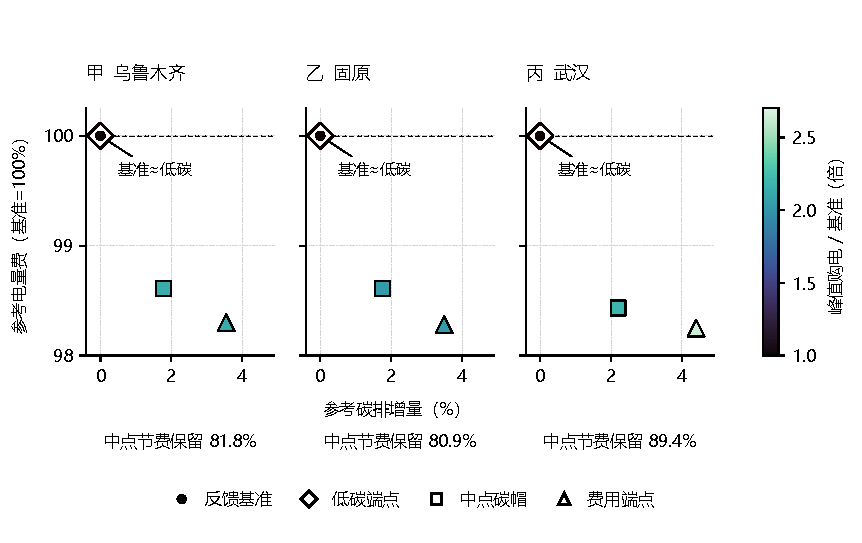
\includegraphics[width=\linewidth]{paper_r2/tradeoff_paper/cost_carbon.pdf}
\caption{三城登记方案的费用、碳排与峰值取舍。图示固定资产实际点，颜色表示峰值与各自基准的比值；中点节费保留率的分母为费用端点相对基准的节省额。}
\label{fig:cost-carbon}
\end{figure}

优化点为固定资产问题的登记容差内最优调度。中点碳帽将电量费端点相对基准的增排约减半，保留80.92\%--89.44\%的降费；对应相对基准增排1.75\%--2.20\%。图\ref{fig:cost-carbon}同步呈现峰值占用，中点为基准的2.04--2.21倍，为联合设置碳帽与配电容量提供依据。
